\section{Addendum to the system documentation}

\subsection{Business class diagram}
\label{subsec:fachklassendiagramm}

Figure \ref{figure:fachklassen} represents an overview of the application's core business classes. Since JavaScript is not used as a class-oriented language, these aren't classes in the narrow sense. A UML class is used for a JavaScript function, local variables for its attributes. In order to implement class methods, the corresponding functions are added to the function's prototypes. An UML association means that the \enquote{class} - in fact a function - calls another \enquote{class} in one of its methods.

The diagram illustrates how business classes behave vis-\'{a}-vis each other. The leftmost controllers access the Mustache views, who in their turn retrieve their data from the models. Independently from the business classes, the {\fontfamily{pcr}\selectfont ConflictDetector} is called through input from the database. In turn, it may call the {\fontfamily{pcr}\selectfont ConflictPresenter} in order to display any conflicts, or it may call the {\fontfamily{pcr}\selectfont ConflictResolver} in order to resolve them. For this purpose, the latter needs data from a {\fontfamily{pcr}\selectfont NoteView} and the {\fontfamily{pcr}\selectfont NotesCollection}. The {\fontfamily{pcr}\selectfont ConflictResolver} can also be called by a {\fontfamily{pcr}\selectfont NotesView} in order to display write conflicts.

\medskip
\begin{figure}[H] 
  \begin{center}
  \includegraphics[width=\textwidth]{grafik/Fachklassendiagramm} 
  % width=\textwidth,height=\textheight,keepaspectratio
  \end{center}
  \caption{Business class diagram}
  \label{figure:fachklassen}
\end{figure}





\subsection{Abstraction of basic database operations}

\lstset{language=javascript}
\medskip 
\begin{lstlisting}[label=code:resources, caption=Extract from {\fontfamily{pcr}\selectfont /\_attachments/app/lib/resources.js}]
var Resources = function(app, couchapp) {
  this.helpers({
    new_object: function(kind, callback) {
      this.partial(template_file_for(kind, 'new'), callback);
    },
    \\ [...]
    
    load_object_view: function(kind, id, callback){
      var context = this;
      couchapp.db.openDoc(id, {
        success: function(doc) {
          var _prototype = eval(kind);
          var view_prototype = eval(kind + 'View');
          var view = new view_prototype(new _prototype(doc));
          if(doc) {            
            callback(view);            
          } else {
            context.flash = {message: kind + ' with ID "' + id + '" not found.', type: 'error'};
          }
        },
        error: function() {
          context.notFound();
        }
      });
    },

    \\ [...]
  });
};
\end{lstlisting}



\subsection{Indentation of an outline's line}


\lstset{language=html}
\medskip 
\begin{lstlisting}[label=code:outline-indent, caption=Line with child nodes]
<li class="edit-note" id="edit_note_2">
  <form class="edit-note" action="#/notes/2" method="put" accept-charset="utf-8">
    <span class="space">&nbsp;</span>
    <a class="image">&nbsp;</a>
    <textarea class="expanding" id="edit_text_2" name="text">Some text</textarea>
    <input type="submit" value="Save" style="display:none;"/>
  </form>

  <ul class="indent">
    <li class="edit-note" id="edit_note_2a">
      <form class="edit-note" action="#/notes/2a" method="put" accept-charset="utf-8">
        <span class="space">&nbsp;</span>
        <a class="image">&nbsp;</a>
        <textarea class="expanding" id="edit_text_2a" name="text">More text</textarea>
        <input type="submit" value="Save" style="display:none;"/>
      </form>
    </li>
  </ul>
</li>
\end{lstlisting}




\subsection{Rendering an outline's lines}

\lstset{language=javascript}
\medskip 
\begin{lstlisting}[label=code:rendernotes, caption=Extract from {\fontfamily{pcr}\selectfont /\_attachments/app/helpers/note\_element.js}]
renderNotes: function(context, notes, counter){
  if (notes.notes.length == 0) return;
  if (notes.notes.length == 1) {
    context.unbindSubmitOnBlurAndAutogrow();
    context.bindSubmitOnBlurAndAutogrow();
    $('#spinner').hide();
    context.i = 0;
  }
  if(typeof(context.i)=="undefined"){
    context.i = counter;
  } else {
    context.i = context.i-1;
  }
  var note_object = notes.findById(this.id());
  var child_object = note_object.firstChildNoteObject(notes.notes);
  var next_object = note_object.nextNoteObject(notes.notes);
  
  notes.notes = notes.notes.remove(note_object);
  
  if(typeof(child_object)!="undefined"){
    this.renderFollowingNote(context, child_object, function(child){
      child.renderNotes(context, notes);
    });
  } 
  if(typeof(next_object)!="undefined"){
    this.renderFollowingNote(context, next_object, function(next){
      next.renderNotes(context, notes);
    });
  }
  if(typeof(next_object)=="undefined" && typeof(child_object)=="undefined"){
    context.unbindSubmitOnBlurAndAutogrow();
    context.bindSubmitOnBlurAndAutogrow();
  }
},

renderFollowingNote: function(context, note_object, callback){
  var this_note = this;
  context.partial('app/templates/notes/edit.mustache', {_id: note_object._id, text: note_object.text}, function(html) {
    if(typeof note_object.parent_id != "undefined"){
      $(html).appendTo(this_note.note_target.closest('li')).wrap('<ul class="indent"></ul>');
      callback(this_note.firstChildNote());
    } else {
      $(html).insertAfter(this_note.note_target.closest('li'));
      callback(this_note.nextNote());        
    }
  });
}
\end{lstlisting}




\subsection{Monitoring the database for changes by others}

\lstset{language=javascript}
\medskip 
\begin{lstlisting}[label=code:changesfeed, caption= {\fontfamily{pcr}\selectfont /\_attachments/app/helpers/replication\_helpers.js}]
checkForUpdates: function(couchapp){
  var context    = this;
  var source     = context.getLocationHash();
  var url        = config.HOST + '/' + config.DB + 
                   '/_changes?filter=doingnotes/changed&source=' + source;   
  
  if(context.getOutlineId()){ 
    $.getJSON(url, function(json){
      var since = json.last_seq;
      var xmlhttp = new XMLHttpRequest();
      xmlhttp.onreadystatechange=function() {
        if(xmlhttp.readyState == 3){
          if(xmlhttp.responseText.match(/changes/)){
            var lines = xmlhttp.responseText.split("\n");
            if(lines[lines.length-2].length != 0){ 
              lines = lines.remove("");
              $.each(lines, function(i, line){
                context.parseLineAndShowChangesWarning(context, couchapp, line, lines);
              });
            }
          }
          if(xmlhttp.responseText.match(/last_seq/)){
            Sammy.log('Timeout in checkForUpdates:', xmlhttp.responseText)
          }
        }
      }
      xmlhttp.open("GET", url+ '&feed=continuous&heartbeat=5000&since=' +since, true);
      xmlhttp.send(null);
    });
  }
}
\end{lstlisting}








\subsection{Patch for CouchDB's changes filter}
\label{subsec:changes-patch}


The function {\fontfamily{pcr}\selectfont make\_filter\_fun} creates a function that loads the corresponding document for each line in the changes feed. With the aid of the document's JSON representation, the indicated filter function can decide whether the line should be included in the returned changes feed. The {\fontfamily{pcr}\selectfont \_conflicts} array is added to the JSON object in line \ref{lst:addtopatch}, which can then be used by filter functions.




\lstset{language=erlang}
\medskip
\begin{lstlisting}[label=code:changes-patch,caption=Function {\fontfamily{pcr}\selectfont make\_filter\_fun},escapeinside={@}{@}]
make_filter_fun(Req, Db) ->
    Filter = couch_httpd:qs_value(Req, "filter", ""),
    case [list_to_binary(couch_httpd:unquote(Part))
            || Part <- string:tokens(Filter, "/")] of
    [] ->
        fun(DocInfos) ->
            [{[{rev, couch_doc:rev_to_str(Rev)}]} ||
                #doc_info{revs=[#rev_info{rev=Rev}|_]} <- DocInfos]
        end;
    [DName, FName] ->
        DesignId = <<"_design/", DName/binary>>,
        DDoc = couch_httpd_db:couch_doc_open(Db, DesignId, nil, []),
        #doc{body={Props}} = DDoc,
        couch_util:get_nested_json_value({Props}, [<<"filters">>, FName]),
        fun(DocInfos) ->
            Docs = [Doc || {ok, Doc} <- [
                @\label{lst:addtopatch}@{ok, Doc} = couch_db:open_doc(Db, DInfo, [deleted, conflicts])
                || DInfo <- DocInfos]],
            {ok, Passes} = couch_query_servers:filter_docs(Req, Db, DDoc, FName, Docs),
            [{[{rev, couch_doc:rev_to_str(Rev)}]}
                || #doc_info{revs=[#rev_info{rev=Rev}|_]} <- DocInfos, 
                Pass <- Passes, Pass == true]
        end;
    _Else ->
        throw({bad_request, 
            "filter parameter must be of the form `designname/filtername`"})
    end.  
\end{lstlisting}

For testing purposes a design document was added to the test database. This document contains a list function returning all conflicting documents.

\lstset{language=javascript}
\medskip
\begin{lstlisting}[label=code:changes-patch-test,caption=Test for the function in listing \ref{code:changes-patch-test}]
var ddoc = {
  _id : "_design/changes_filter",
  "filters" : {
    "conflicted" : "function(doc, req) { return (doc._conflicts);}",
  }
}

var id = db.save({'food' : 'pizza'}).id;
db.bulkSave([{_id: id, 'food' : 'pasta'}], {all_or_nothing:true});

req = CouchDB.request("GET", "/test_suite_db/_changes?filter=changes_filter/conflicted");
resp = JSON.parse(req.responseText);
T(resp.results.length == 1);
\end{lstlisting}





\subsection{HTML file for executing the unit tests}


\lstset{language=html}
\medskip 
\begin{lstlisting}[label=code:jspec-index,caption={\fontfamily{pcr}\selectfont /\_attachments/spec/index.html}]
<html>
  <head>
    <link rel="stylesheet" href="jspec/jspec.css" type="text/css"/>
    <script src="../../vendor/jquery/_attachments/jquery.js"></script>
    <script src="jspec/jspec.js"></script>
    <script src="jspec/jspec.jquery.js"></script>
    <script src="jspec/jspec.xhr.js"></script>
    <script src="../app/lib/lib.js"></script>
    <script src="../app/lib/resources.js"></script>
    <script src="../config/config.js"></script>
    <script src="../app/helpers/key_events.js"></script>
    <script src="../app/helpers/note_element.js"></script>
    <script src="../app/helpers/outline_helpers.js"></script>
    <script src="../app/models/note.js"></script>
    <script src="../app/models/outline.js"></script>
    <script src="../app/models/note_collection.js"></script>
    <script>
      function runSuites() {
        JSpec
        .exec('note_element_spec.js')
        .exec('inserting_note_element_spec.js')
        .exec('indenting_note_element_spec.js')
        .exec('unindenting_note_element_spec.js')
        .exec('focusing_note_element_spec.js')
        .exec('rendering_note_element_spec.js')
        .exec('outline_helpers_spec.js')
        .exec('outline_spec.js')
        .exec('note_spec.js')
        .exec('note_collection_spec.js')
        .exec('resources_spec.js')
        .exec('lib_spec.js')
        .exec('conflict_spec.js')
        .run({failuresOnly: true, fixturePath: 'fixtures'})
        .report();
      }
    </script>
  </head>
	<body class="jspec" onLoad="runSuites();">
		<div id="jspec"></div>
	</body>
</html>
\end{lstlisting}










\subsection{Test suite for CouchDB's JavaScript API}
\label{subsec:httpapi}

\subsubsection{Extract from CouchDB's JavaScript API}

\lstset{language=javascript}
\medskip 
\begin{lstlisting}[label=code:httpapi, caption=Extract from {\fontfamily{pcr}\selectfont /share/www/script/jquery.couch.js}]
(function($) {
  \\ [...]
  $.extend($.couch, {
    \\ [...]
    db: function(name) {
      \\ [...]
      return {
        \\ [...]
        removeDoc: function(doc, options) {
          ajax({
              type: "DELETE",
              url: this.uri +
                   encodeDocId(doc._id) +
                   encodeOptions({rev: doc._rev})
            },
            options,
            "The document could not be deleted"
          );
        }
        \\ [...]
      };
    }
    \\ [...]
  });
})(jQuery);
\end{lstlisting}


\subsubsection{Test for listing \ref{code:httpapi}}
\label{subsec:testsuite-jspec-code}

\medskip
\begin{lstlisting}[label=code:httpapitest, breaklines=true, caption=Extract from {\fontfamily{pcr}\selectfont /share/www/spec/jquery\_couch\_3\_spec.js}]
describe 'jQuery couchdb db'
  \\ [...]
  
  before_each
    db = $.couch.db('spec_db');
    db.create();
  end
  
  after_each
    db.drop();
  end

  describe 'removeDoc'
    before_each
      doc = {"Name" : "Louanne Katraine", "Callsign" : "Kat", "_id" : "345"};
      saved_doc = {};
      db.saveDoc(doc, {
        success: function(resp){
          saved_doc = resp;
        },
        error: function(status, error, reason){errorCallback(status, error, reason)}
      });
    end
    
    it 'should result in a deleted document'
      db.removeDoc({_id : "345", _rev : saved_doc.rev}, {
        success: function(resp){
          db.openDoc("345", {
            error: function(status, error, reason){
              status.should.eql 404
              error.should.eql "not_found"
              reason.should.eql "deleted"
            },
            success: function(resp){successCallback(resp)}
          });
        },
        error: function(status, error, reason){errorCallback(status, error, reason)}
      });
    end
  
    it 'should return ok true, the ID and the revision of the deleted document'
      db.removeDoc({_id : "345", _rev : saved_doc.rev}, {
        success: function(resp){
          resp.ok.should.be_true
          resp.id.should.eql "345"
          resp.rev.should.be_a String
          resp.rev.length.should.be_at_least 30
        },
        error: function(status, error, reason){errorCallback(status, error, reason)}
      });
    end
      
    it 'should record the revision in the deleted document'
      db.removeDoc({_id : "345", _rev : saved_doc.rev}, {
        success: function(resp){
          db.openDoc("345", {
            rev: resp.rev,
            success: function(resp2){
              resp2._rev.should.eql resp.rev
              resp2._id.should.eql resp.id
              resp2._deleted.should.be_true
            },
            error: function(status, err, rsn){errorCallback(status, err, rsn)}
          });
        },
        error: function(status, error, reason){errorCallback(status, error, reason)}
      });
    end
    
    it 'should alert with an error message prefix'
      db.removeDoc({_id: "asdf"});
      alert_msg.should.match /The document could not be deleted/
    end
  end

  \\ [...]
end
\end{lstlisting}







\newpage
\subsection{Screenshots from the AWS management console}
\label{subsec:aws}

\begin{figure}[H] 
  \begin{center}
    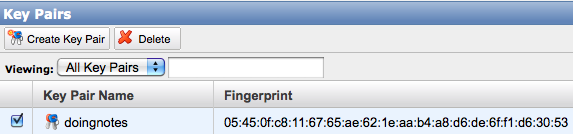
\includegraphics[width=\textwidth]{grafik/aws-key-pair} 
  \end{center}
  \caption{AWS: key pair for authentification}
  \label{fig:aws-key}
\end{figure}

\begin{figure}[H] 
  \begin{center}
    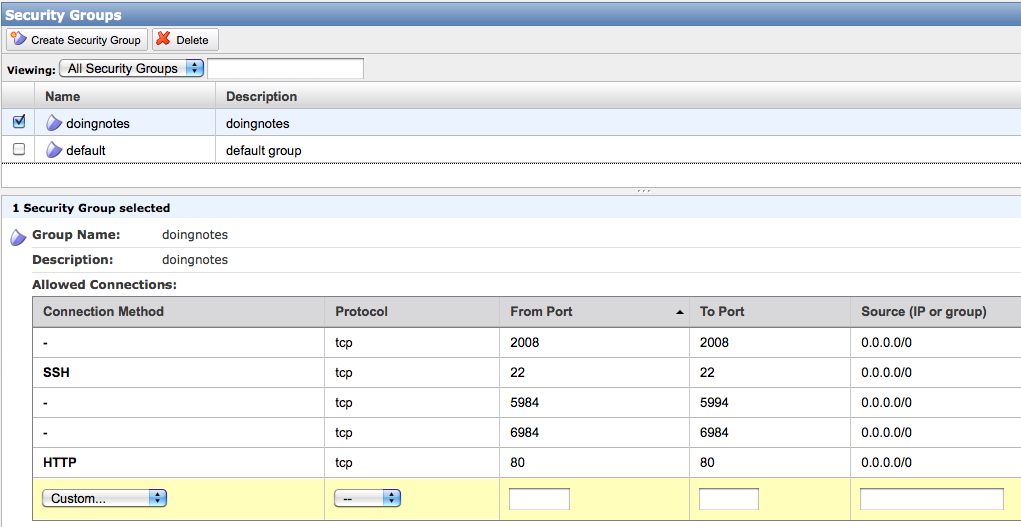
\includegraphics[width=\textwidth]{grafik/aws-security-group} 
  \end{center}
  \caption{AWS: opening ports using security groups}
  \label{fig:aws-group}
\end{figure}

\begin{figure}[H] 
  \begin{center}
    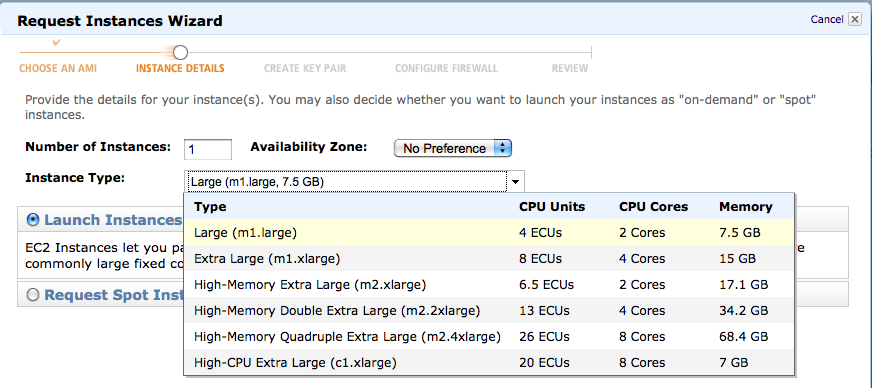
\includegraphics[width=\textwidth]{grafik/aws-select-size} 
  \end{center}
  \caption{AWS: choosing instance capacity}
  \label{fig:aws-size}
\end{figure}

\begin{figure}[H] 
  \begin{center}
    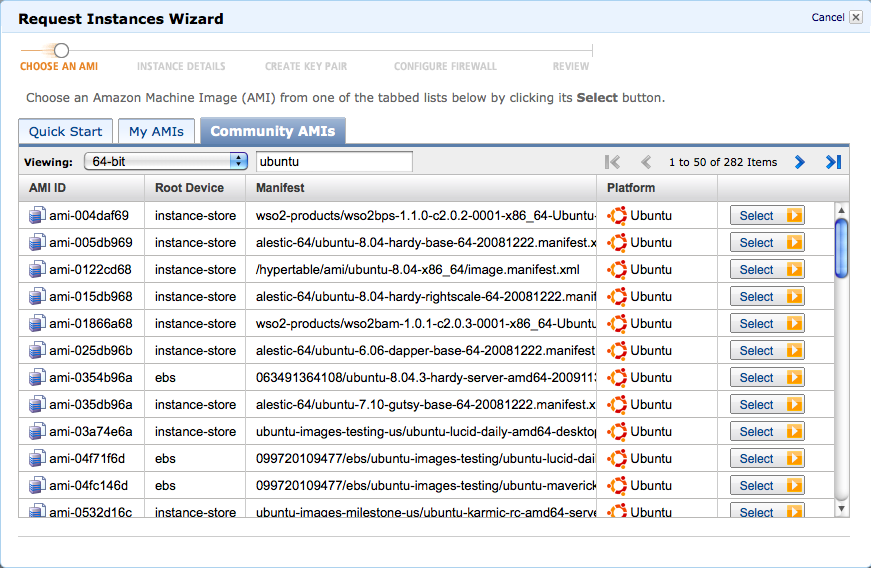
\includegraphics[width=\textwidth]{grafik/aws-select-AMI} 
  \end{center}
  \caption{AWS: choosing an Amazon Machine Image}
  \label{fig:aws-ami}
\end{figure}

\begin{figure}[H] 
  \begin{center}
    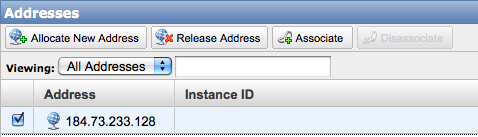
\includegraphics[width=\textwidth]{grafik/aws-ip} 
  \end{center}
  \caption{AWS: Elastic IP set-up}
  \label{fig:aws-ip}
\end{figure}

\begin{figure}[H] 
  \begin{center}
    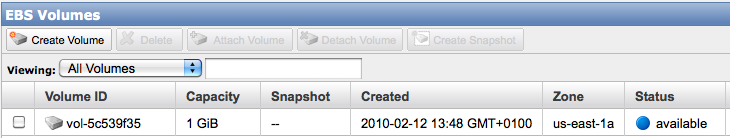
\includegraphics[width=\textwidth]{grafik/aws-ebs-volume} 
  \end{center}
  \caption{AWS: EBS volume set-up}
  \label{fig:aws-ebs}
\end{figure}


\begin{figure}[H] 
  \begin{center}
    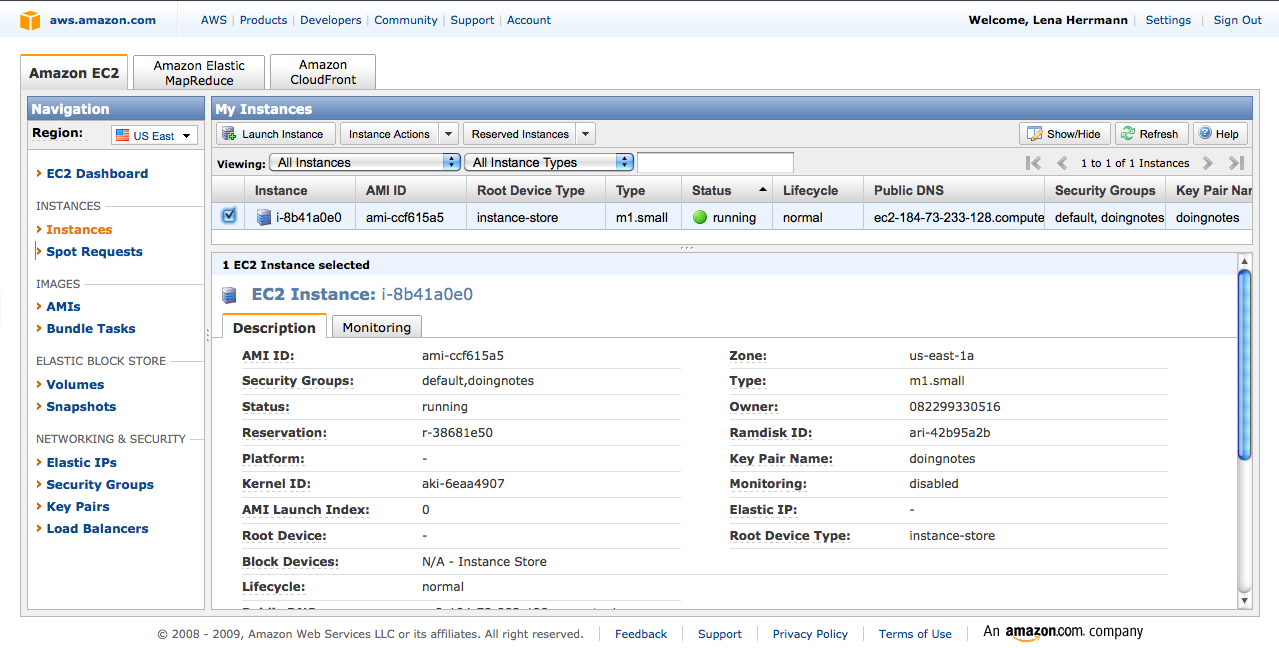
\includegraphics[width=\textwidth]{grafik/aws-ec2-management-console} 
  \end{center}
  \caption{AWS: running EC2 instance}
  \label{fig:aws-console}
\end{figure}